The case study leverages Matrix as a secure communication channel and Paragon as the Information-Flow Control tool for securing the endpoints. 

This chapter consists of two parts. The first part will provide an evaluation of the Matrix security and relies on the paper \emph{SoK: Secure Messaging} \cite{sok} and \emph{The Olm Cryptographic Review} by NCC Group \cite{ncc}. 

The second part provides a preliminary analysis of some IFC tools, the selection of Paragon and the rationale behind it.

% This chapter will present the criteria \emph{evaluation of Matrix security model}

\section{Evaluation of Matrix security model}\label{evaluationofmatrix}
The security of matrix will be evaluated in the context of secure messaging. An evaluation framework has been proposed in the paper \emph{SoK: Secure messaging} which the evaluation will be loosely based on. 

The evaluation framework covers several areas with \emph{conversation security} being the most relevant for this evaluation. The area \emph{conversation security} describes three categories; \emph{Security and Privacy}, \emph{Adoption}, and \emph{Group Chat}. Obviously the most relevant category for the evaluation is \emph{Security and Privacy}

\subsection{Threat model}
For secure messaging the evaluation framework defines a threat model with three types of adversaries. Note that an adversary can be of several types:

\begin{itemize}
	\item \emph{Local adversary:} The adversary is in control of the local network.
	\item \emph{Global adversary:} The adversary is in control of great portions of the Internet 
	\item \emph{Service providers:} A potential adversary for messaging systems with centralized infrastructure.
\end{itemize}

In the messaging system the adversary may be a participant with the following properties:

\begin{itemize}
	\item An adversary can start a conversation.
	\item An adversary can send messages.
	\item An adversary can perform any other action that a participant is capable of.
\end{itemize}

Furthermore it is assumed that the system's endpoints are secure \cite{sok}.

This evaluation will inherit the described threat model.

\subsection{The Signal Protocol}
Matrix provides end-to-end encryption by using the Olm and Megolm library with the former being an implementation of the Double Ratchet algorithm also known as the Signal Protocol, and the latter being the algorithm used for group chat. 

Olm is used for securely exchanging message keys/session keys during group chat and is vital part of the end-to-end encryption in Matrix.

Before the Matrix protocol is evaluated the Signal Protocol will be considered. The Signal Protocol is described in section xx. 

Section xx provides a list of security properties relevant for \emph{conversation security}. These security properties is used for evaluating a secure messaging protocol such as the Signal Protocol.
%Any messaging application that provides end-to-end encryption is likely an implementation of  the protocol 

The table below shows an evaluation of the Signal Protocol (previously known as TextSecure) \cite{sok}. 

\begin{figure}[H]
	\hspace*{-1.7cm} 
	\centering
	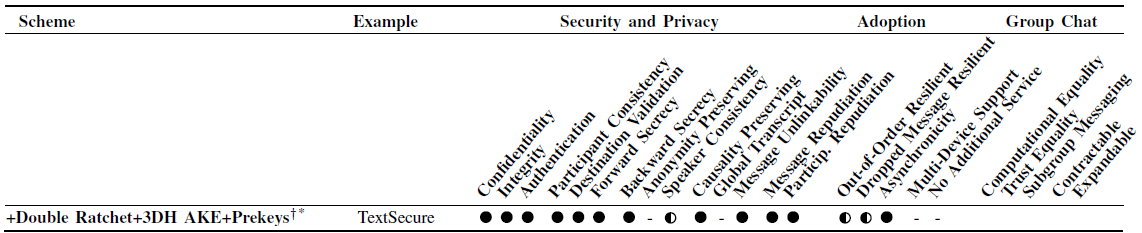
\includegraphics[width=16cm]{figures/framework_signal.png}
	\caption{Evaluation of Signal (TextSecure) \cite{sok}.}
	\label{fig:framework_signal}
\end{figure}


%Explain how they provide the properties or why they don't


\subparagraph{Confidentiality} When a message is sent using the Signal Protocol then only the intended recipient can read the message. The senders sending ratchet and receivers receiving ratchet will derive the same message key hence only the two parties will be able to encrypt the messages. 

\subparagraph{Integrity} The receiver will only accept a message if it is successfully decrypted hence if in transit a message was modified then the message would be rejected.

\subparagraph{Authentication} The decryption of a message also gives authentication guarantees since only the intended recipient could compute the message key.

\subparagraph{Forward secrecy} The symmetric ratchet ensures forward secrecy. If a chain session key is compromised then the previous keys can not be generated since the ratchet is one way cryptographic hash function hence secrecy is provided for all previous send messages.  

\subparagraph{Backward secrecy} Diffie-Hellman ratchet have the self-healing property and will generate a new chain session key for the symmetric ratchet hence if a chain key is compromised then secrecy for future messages is still provided because a new chain ratchet key will be generated.

\subparagraph{Anonymity preserving}

Anonymity preservation is lost in the Signal Protocol since the initial key agreement requires long-term public keys hence making them observable during Triple-DH. However \textbf{\emph{participant consistency}} is provided by Triple-DH \cite{sok}. %How?
%Without participant consistency, identity misbinding attacks might be possible. Unknown key share attack

\subparagraph{Speaker consistency}
This property is partially provided through the key evolution of the ratchets. If a message is dropped then it is not possible to generate message keys for future messages. This also makes the protocol have the property \textbf{\emph{Causality Preserving}} and partially have the property \emph{\textbf{Dropped message resilence}}. It will also not go unnoticed if a message is received out of order since this will result in the message's key being an unexpected key. Hence the recipient have to store expired keys to decrypt delayed messages. This makes the property \emph{\textbf{Out-of-order resilient}} only partially provided \cite{sok}.

\subparagraph{Global transcript} 
In an asynchrounous messaging protocol there is no global transcript. Both participants have to be online to receive messages hence the participants will not have all the messages if one of them is offline. This is a result of having the \textbf{\emph{Asynchronicity}} property.

\subparagraph{Deniability properties}

Since the ratchet session keys are used for encrypting messages and not the long-term public keys the properties \textbf{\emph{Message unlinkability}} and \textbf{\emph{Message repudiation}} are provided. 


\subparagraph{Other properties}

\begin{itemize}
	\item \textbf{\emph{Participant repudiation}}. Triple-DH achieves full participant repudiation since anyone can forge a transcript between any two participants \cite{sok}.
	\item \textbf{\emph{Destination validation}}. The Deffie-Hellman ratchet provides this property since the recipients public key is used to generate the chain key \cite{sok}. % Is this true?
\end{itemize}


The evaluation shows that several security properties are provided with the important ones being confidentiality, integrity, authentication, forward secrecy, backward secrecy. 

Furthermore a formal analysis have been made on the Signal Protocol that proves the protocol is free from any major flaws and it satisfy the following security properties; confidentiality, authentication and secrecy \cite{Signal}. 

\paragraph{Application variants}

The Signal Protocol is a secure messaging protocol and have been extensively studied including proof that the standard security properties are assured. 

The Olm library used by Matrix is a variant of the Signal Protocol. There is no implementation analysis of the Olm library hence there is no guarantee that all the security properties defined in xx is inherited by Olm. Nevertheless it is assumed that Olm inherits the above properties.

The further evaluation relies upon the the security assessment of Matrix. 


\subsection{Matrix protocol}\label{matrixeval}

As described in section xx \emph{rooms} are a fundamental part of Matrix' architecture. There can be multiple participants in a room hence the support for secure group conversation is required. 

Olm (and the Signal Protocol it is based on) is ideally meant for two party communication.
Group conversation could be supported with a näive variant of Olm. In a group with N participants each participant would establish a secure Olm session with every other participant. When a message is send each message would then have to be encrypted N times. This solution would scale poorly if N was a large number. This was the motivation for introducing Megolm.

\paragraph{Megolm}

Megolm is a multicast encryption solution \cite{sok}.Each sender has a sender ratchet (Megolm Ratchet). Each recipient has a corresponding receiving ratchet for each sender. So if there are N participants in a group then each participant will have N-1 receiving ratchets. Figure \ref{fig:megolm} illustrates the setup with three participants. 

\begin{figure}[H]
	\hspace*{-1cm} 
	\centering
	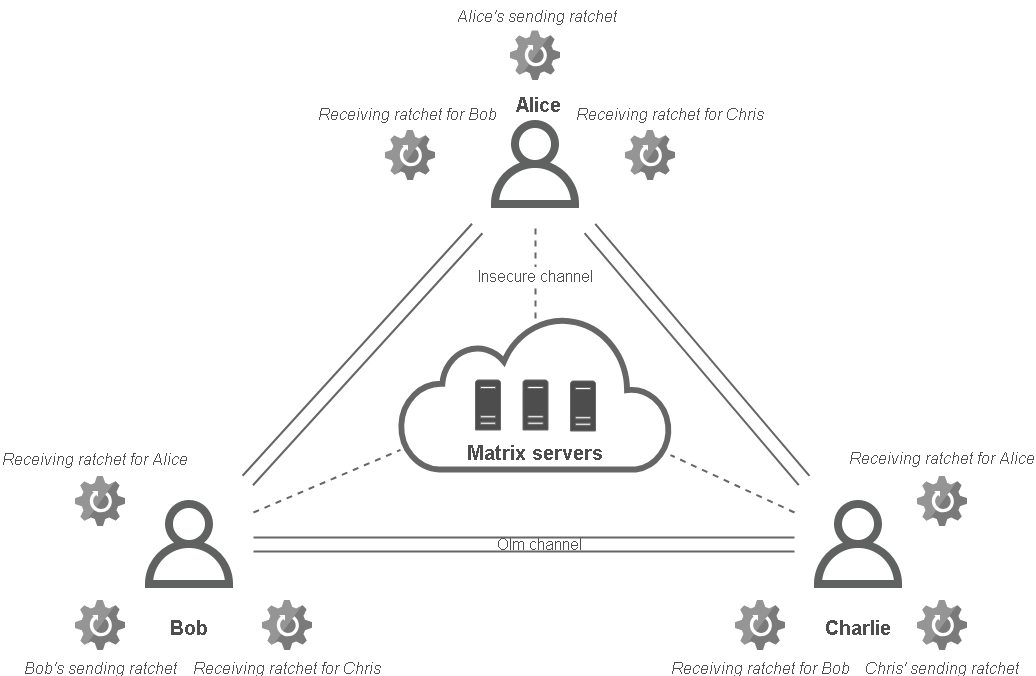
\includegraphics[width=14cm]{figures/megolm_conceptual.png}
	\caption{Conceptual model of Megolm with three participants.}
	\label{fig:megolm}
\end{figure}

When a session is started a sender will send his initial ratchet key to each recipient, so that the sender ratchet and each recipients ratchet are in sync. This key exchange happens over a secure communication channel (Olm). Furthermore there is send N-1 initial messages when a session is initiated. Until a new session is started no further session keys are exchanged and the corresponding message keys are generated by incrementing the ratchet.

When a sender sends a message a message key is generated from the ratchet key and the message is encrypted using that message key. The message will be signed so the recipient will know which sender the message is from and which ratchet to utilize. %(not with a long-term I guess? hence providing deniability)
The message  is then send to the server which relays the message to all recipients over an insecure channel. When they receive the message the same message key is generated using the corresponding receiver ratchet and the message is decrypted. 

When a new participant joins the latest ratchet key would then be shared by each participant over Olm (or an earlier one if he should have access to historical conversation). 

When a participant leaves a new session would be initiated yielding in refreshing the ratchet keys hence not making it possible for that ex-participant to decrypt any further messages.




% add figures for naive olm and multicast encryption solution

The Matrix Protocol will be evaluated in the context of Megolm. The evaluation of the Matrix protocol heavily relies on the security assessment by NCC.


\subsubsection{Evaluation}

The Matrix Protocol provides several security properties shown in the table xx. 

It is worth mentioning that there is a trade-off between security and usability which must be decided at application layer. The most secure configuration would come at the cost of usability and performance.    
\begin{itemize}
	\item \emph{Usability}. From a users point of view it would be nice to have the possibility to load historical conversation instead of having to keep full history locally. Matrix supports multiple devices and if a participant adds another device at some later point it makes sense to load the participants historical conversation into the device. From a security perspective this would mean that the \emph{initial ratchet state} is stored and is send to the new device so every message key can be generated. This certainly goes against the principle of forward secrecy. The most secure configuration would not store the \emph{initial ratchet state} hence satisfy forward secrecy thus disable the described usability feature \cite{ncc} \cite{megolm}.
	\item \emph{Performance}. When a megolm session is initialized there is an initial burst of messages to exchange the initial ratchet key which is then stored in a \emph{initial ratchet state} value at each recipient. If this key is compromised then any future key can be generated for that session. To satisfy backward secrecy this would mean initiating a new session for each message which would trigger a burst of messages to exchange the ratchet key \cite{ncc} \cite{megolm}. This would scale poorly for a large group or when sending large-sized messages. 
\end{itemize} 


\begin{figure}[H]
	\hspace*{-1.7cm} 
	\centering
	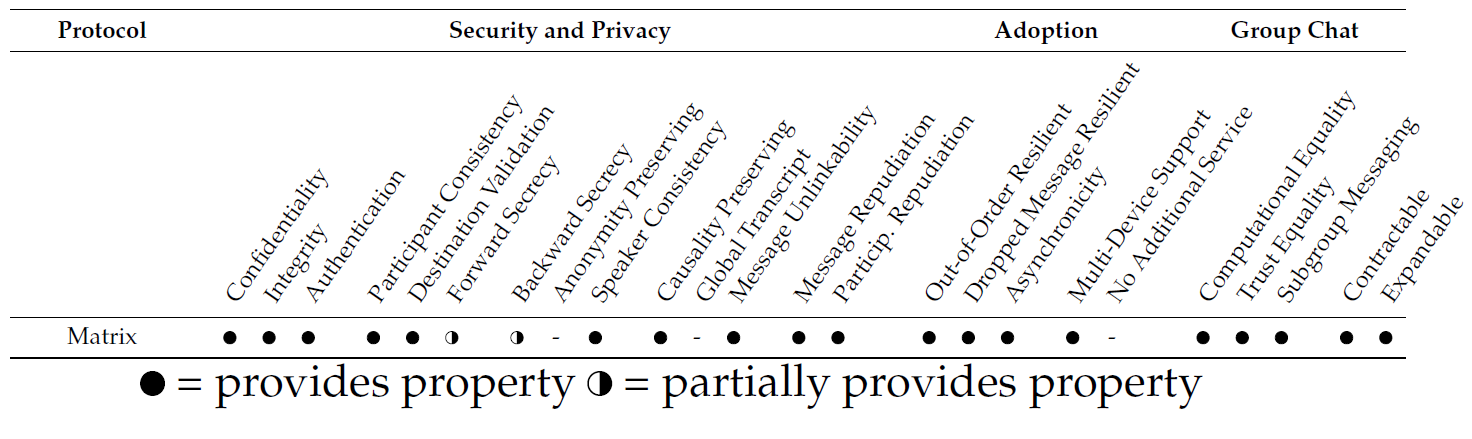
\includegraphics[width=16cm]{figures/framework.png}
	\caption{Evaluation of Matrix Security.}
	\label{fig:framework}
\end{figure}

Some of the security properties in the table are briefly examined.

\subparagraph{Confidentiality} When a message is send it is encrypted and can only be decrypted by the intended recipients who has the corresponding ratchet session key received over an Olm channel. 

\subparagraph{Integrity} The receiver will only accept a message if it is successfully decrypted hence if in transit a message was modified then the message would be rejected. 


\subparagraph{Forward secrecy} Each participant keeps a \emph{initial ratchet state} which holds the earliest ratchet session key for a session. This clearly violates forward secrecy since every message can be decrypted if the \emph{initial ratchet state} value is compromised. However it is a deliberate trade-off for usability to enable historical conversation and storing the value is optional. Since this is an optional feature the forward secrecy is partially provided \cite{ncc}. 

%From NCC

\subparagraph{Backward secrecy} If a ratchet key is compromised then an adversary can generate every message key from that point on hence intercept any message that sender sends to the group. This can be prevented strictly by starting a new session with every send message however it would not be possible to keep conversation history (only locally when data is encrypted). Hence the property is only partially provided \cite{ncc}.

% From NCC


\subparagraph{Speaker consistency}

There is no guarantee for speaker consistency. A well known problem of multi-cast encryption group chat is transcript inconsistency. A sender may send different messages to different recipients. However it requires that the server is in collusion with the sender. This also applies to \emph{\textbf{Causality preserving}} \cite{ncc}.


\paragraph{Other properties}

The multi-cast encryption design does not provide \emph{participant consistency} \cite{sok}.

The properties \emph{Dropped message resilence} and \emph{Out-of-order resilient} are provided by keeping track of ratchet indices. 

Several properties are inherited from the secure key exchanging channel provided by Olm while other properties are inherited because of asynchronicity of the Megolm protocol.

\begin{itemize}
	
	\item \emph{Authentication} is provided by Olm since the ratchet session key is send to the recipient through an Olm channel or else the message key could not be derived.
	\item \emph{Destination validation}. The ratchet session key is exchanged over a secure Olm channel hence only the intended recipient could decrypt it.
	\item \emph{Anonymity preserving} is not provided since Olm requires the long-term public key in the initial key exchange.
	\item \emph{Global transcript} is also not provided because of the asynchronous nature of the Megolm protocol.  
	\item \emph{Asynchronicity} is obviously provided.
	\item \emph{Deniability} properties are inherited from Olm as well.
\end{itemize}

All properties related to group chat are also provided. Although they are additional features and not related to security. 


\paragraph{Other findings}

\subparagraph{Message Replays}

Matrix allows decryption of a message multiple times hence it is vulnerable to replay attacks. Replay attacks are handled at the application layer. Whenever a message is decrypted a message index is generated and stored. If the exact message is decrypted again the same message index will be generated and can be compared to the stored message index making the replayed message invalid. 

\subparagraph{Unknown key-share attack}

The \emph{Unknown key-share attack}\footnote{https://en.wikipedia.org/wiki/Unknown\_key-share\_attack} is a vulnerability found with a high risk in Megolm. The vulnerability is inherited from Olm and occurs after the initial message in Triple-DH. 

The vulnerability has been mitigated at the application layer by providing a unique identifier for the sender and receiver into each message and then checking the values when decrypted \cite{ncc}.

\paragraph{Recent research}
The way backward secrecy would be provided in Matrix is computationally expensive. Recent research has proposed solutions with early implementations for these problems with IETF leading the research on the standard on \emph{Messaging Layer Security}. Matrix has expressed awareness of the protocol and a possibility of adaption in the future.

\subsection{End-to-end security}

Section xx describes Matrix long-term goal as being a generic HTTP messaging API. It could be utilized for any kind of data exchange in a system or between multiple systems.

A system using the Matrix Protocol for exchanging data would benefit from the security properties found in the evaluation yet the system-wide security or end-to-end security would be incomplete an further measures must be taken. Such system might demand confidentiality and integrity throughout the system yet the system as a whole would have a different threat model than the one described for a secure messaging system hence no guarantee of confidentiality or integrity beyond the endpoints in end-to-end encryption. 

The following figure depicts how end-to-end encryption might be inadequate in such system. 

\begin{figure}[H]
	\centering
	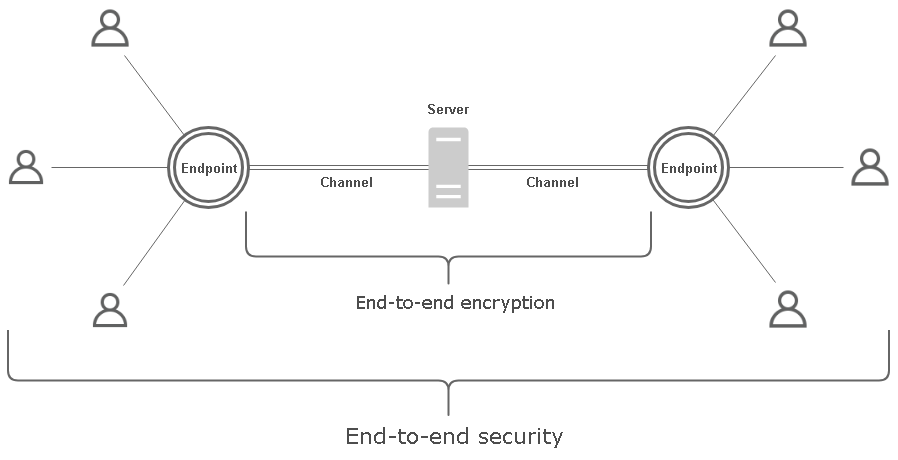
\includegraphics[width=12cm]{figures/e2esecurity.png}
	\caption{End-to-end security.}
	\label{fig:e2esecurity}
\end{figure}

As the system depicts there might be several principals accessing the endpoint. Each principal could retrieve some information possibly protected with access control. Assume that the information resting at the endpoint is of confidential nature; access could still be granted with no respect of the confidentially of that information. There clearly lack a mechanism of specifying what information is confidential or public and where it may flow under what conditions.  
\\
\\
Matrix identifies IoT as another use case. A person can have several devices for health tracking, entertainment and so on. The data from the devices are send to vendors - a device might send data to several vendors. Ultimately this give a fragmentation of the person's own data with it being placed at several vendors data back-end. Matrix proposes a solution where all the device data for a person is synchronized and persisted on Matrix. Vendors would be connected to Matrix. This is depicted in figure \ref{fig:matrix_iot} below. 

\begin{figure}[H]
	\centering
	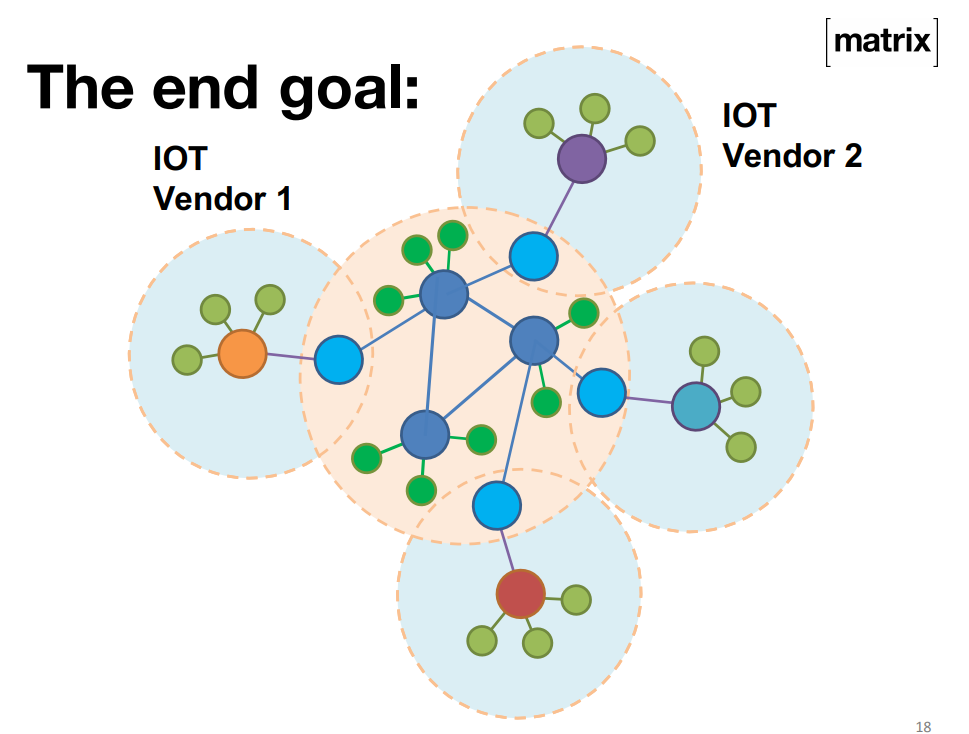
\includegraphics[width=10cm]{figures/matrix_iot.png}
	\caption{End goal for Matrix IoT}
	\label{fig:matrix_iot}
\end{figure}

The data flowing from the sensors to Matrix might be of sensitive nature or the owner might only allow some data to flow to some vendors under specific conditions. This issue related to confidentiality is not addressed by Matrix. 

\subsection{Evaluation summary}

In this section an evaluation of Matrix security was presented. Several security properties are a part of Matrix security model with forward secrecy and backward secrecy being provided depending on the Matrix configuration.

End-to-end encryption is not the end of security. Other security measures must be taken to provide confidentiality and integrity. Information Flow Control is such measure and the next section will present a survey on Information Flow Control.


\newpage
\section{Analysis of IFC Tools}
%Enforcing new session start every time a patient journal is sent. Could it be enforced with IFC?
% Tools issue: java sdk for matrix is beta and not fully implemented. 
% Best supported sdk is for javascript or python. Problem of running javascript code or python code with Paragon (java)
% Maybe better to use JSFlow instead 

% This chapter will present the criteria \emph{Survey of IFC tools and selection of tool}


Different Information-Flow Control tools were considering for the case study. Before developing the prototype several tools were studied. This section describe three of those tools; \emph{Jif}, \emph{Paragon} and \emph{JSFlow}. This section further justify the selection of Paragon.

\subsection{Jif}

Jif is a Java based security-typed programming language that provides information flow control through static enforcement. Jif implements the Decentralized Label Model (DLM) described in section \ref{dlm}. Policies are defined conforming to the DLM. The policies are enforced at compile time with support for enforcement of dynamic policies at runtime. If a Jif program adheres to the specified policies the Jif compiler then compiles it to a secure Java program \cite{jifmanual}. 

A policy is defined by labels and are associated with program variables. A policy can specify multiple principles that have readers or writers. A policy is defined as: 

\begin{lstlisting}[mathescape]
int {Alice$\rightarrow$Bob; Alice$\leftarrow$Bob} x;
\end{lstlisting}

The policy specifies two things; that first part with "$\rightarrow$" expresses \emph{Alice} controls the variable x and the variable can be read by \emph{Bob}, the second part with "$\leftarrow$ expresses that bob can write to it \cite{jifmanual}. 

The following code shows another example:

\begin{lstlisting}[mathescape]
	int {Alice} x;
	int {Alice$\rightarrow$Bob} y;
	x = y; // OK
	y = x; // BAD
\end{lstlisting}


Variable  \emph{x} has a policy that \emph{Alice} controls with no readers. The variable \emph{y} is owned by \emph{Alice} with \emph{Bob} being able to read hence the label is less restrictive than \emph{x}'s label. The compiler allows the \emph{x = y} since \emph{Bob} is specified as a reader for \emph{x}. However the expression \emph{y = x} is illegal since \emph{x} has a stronger policy than y and the explicit flow is caught \cite{jifmanual}.


A important feature for security-typed languages are declassification. Noninterference is too strict for practical programs thus it is necessary to declassify information at times. The following example has two variables with different labels. Variable \emph{x} is more restrictive than \emph{y}; that has \emph{Bob} as a reader. The example depicts an implicit flow: 

\begin{lstlisting}[mathescape]
	void implicitFlow(){
		int {Alice$\rightarrow$} x;
		int {Alice$\rightarrow$Bob} y;
		if (x == 1) { 
			// pc has label {Alice$\rightarrow$}
			y = 0; // BAD
		}
	}
\end{lstlisting}

When the code branches on the if statement the pc has the label \emph{\{Alice$\rightarrow$\}} and the expression \emph{y = 0} becomes illegal since it has the label \emph{\{Alice$\rightarrow$Bob\}} which is less restrictive than the label pc is holding. If for some reason we would want the expression to become valid we would have to declassify it:

\begin{lstlisting}[mathescape]
	void declassificationExample() where authority(Alice) {
		int{Alice$\rightarrow$} x;
		int{Alice$\rightarrow$Bob} y;
		 // PC has label {}
		if (x == 1) {
			 // PC has label {Alice$\rightarrow$}
			declassify({Alice$\rightarrow$} to {Alice$\rightarrow$Bob}) {
				y = 0; // OK
			}
		}
	}
\end{lstlisting}

To be able to declassify it must be through the authority of the owner. This has to be specified at the method definition. When the code branches on the if statement the program counter \emph{pc} has the label \emph{\{Alice$\rightarrow$\}} which can then be declassified to a label as restrictive as \emph{y}'s label \cite{jifmanual} \cite{Srikant}.

Another interesting feature is dynamic labels. Jif provides a run-time library which compares labels at runtime using a syntax that resembles if-statements.
\begin{lstlisting}[mathescape]
	void m(int{*lbl} i, label{} lbl) {
		int{Alice$\rightarrow$} x;
		if (lbl <= new label {Alice$\rightarrow$}) {
			x = i; // OK, since {*lbl} <= {Alice$\rightarrow$}
		}
		else {
			x = 0;
		}
	}
\end{lstlisting}

The parameter variable \emph{i} has the label held by the label \emph{lbl} which would be resolved at runtime. Since the variable \emph{x} has label \emph{\{Alice$\rightarrow$\}} we can allow a flow to that variable as long it is less or equally restrictive. The static analysis of the program will pass and the program will be able to compile.  
%Dynamic label example


Other relevant features that Jif supports are label inference\footnote{http://www.cs.cornell.edu/jif/doc/jif-3.3.0/language.html\#inference} and parameterized classes\footnote{http://www.cs.cornell.edu/jif/doc/jif-3.3.0/language.html\#parameterized-classes}.
\subsection{Paragon}

Paragon is a programming language that extends Java with the ability to express security policies for data. Paragon has similar characteristics to Jif and essentially solving the same problem. Paragon have a different approach to defining information flow policies; \emph{Paralocks} \cite{paralocks} \cite{paragonpaper}.
At the core \emph{Paralocks} is based on the concepts; \emph{actors} and \emph{locks} \cite{paralocks}. An actor is a user with some role. For information can flow to an actor there might be a condition that states; that the actor must be of a specific role. These conditions are represented by boolean variables \emph{locks} and can be modified throughout program execution. These locks are called \emph{parameterized locks} since they are parameterized over actors. Policies are specified by parameterized locks and \emph{actor polymorphism} allows us to reason about all actors \cite{paragonpaper}.


In Paragon policies are immutable and are defined as such:

\begin{lstlisting}
	public static final policy low  = { Object x: };
	public static final policy high = { };
\end{lstlisting}

Policies for \emph{low} and \emph{high} can encoded in different ways. The encoding specifies the most liberal policy that anyone can see the data that has the policy of \emph{low}. The actor is any \emph{Object x} hence anyone can read. The encoding for \emph{high} is the most strict policy and specifies that actors so no one can see the data \cite{paragonprogramming}.

To support a simple declassification mechanism a lock would have to be introduced and the \emph{high} policy definition would have to be redefined:

\begin{lstlisting}
	private lock Declassify;
	public static final policy low  = { Object x: };
	public static final policy high = { Object x: Declassify};
\end{lstlisting} 

The \emph{high} policy now specifies that information can only be read if the \emph{ declassify lock} is open. The following method can now allow declassification:

\begin{lstlisting}
	public static ?low int declassify(?high int x){
		open Declassify { return x; } 
	}
\end{lstlisting} 

The method is a custom declassification method for variables with type \emph{int}. By using Java generics the same method could be used for any type. The \emph{declassify()} method takes a parameter that has the policy \emph{high} and returns the parameter with the lower policy \emph{low}. The method opens the lock hence allowing the value of \emph{x} to be read and returned. 
%Java generics is used to allow declassification of any type.
 
\begin{lstlisting}
publicVariable = declassify(secretVariable); // OK
\end{lstlisting} 
 
 
The example illustrates a simple declassify method however it can be called by anyone. To ensure that only those with the right authority can call it the example could easily be extended with another lock \cite{paralocks}. 

It is possible to support policies at runtime with locks \cite{paragonprogramming}. Suppose we have a customer who buys some software. The software keys should only be given when the customer has paid. We define the following:

\begin{lstlisting}
	public static lock Paid;
	?{customer: } String customerData
	?{customer: Paid} String softwareKey
\end{lstlisting}

When the the customer's payment is processed the lock \emph{Paid} should only be open if the payment is successful. 

\begin{lstlisting}
	public void processPayment() {
		// customer pays for item
		if (paymentSuccessful) { open Paid; } else { ... }
	}
\end{lstlisting}

It is not possible for the compiler to learn the state of the lock \emph{Paid}. By using the lock in a conditional statement the lock will be checked at runtime \cite{paragonprogramming}.

\begin{lstlisting}
	processPayment();
	if (Paid) { customerData = softwareKey; } else { ... }
\end{lstlisting}   

Paragon is a powerful tool for Information-Flow Control and has an interesting policy language with support for expressive dynamic policies. Other relevant features in paragon are policy inference and Java generics.

\subsection{JSFlow}

JSFlow is a tool for tracking information flow in JavaScript web applications. This tool is not a programming language as the two previously described tool but a JavaScript interpreter that supports full non-strict ECMA-262 \cite{jsflowsite}. JSFlow enforces secure information flow through dynamic analysis and can detect explicit and implicit flows. JSFlow uses a program counter \emph{pc} to track the security context. JSFlow defines two built-in security levels; \emph{public} and \emph{secret}, it also supports custom security labels on values. JSFlow allows pure explicit flows by upgrading the security label of the variable being assigned to \cite{jsflowsite}:

\begin{lstlisting}
	high = lbl(true);
	low = high;
\end{lstlisting}
 
The variable \emph{high} is assigned a secret value denoted by the \emph{lbl} function. When \emph{high} is assigned to \emph{low} the security label is upgraded for low. JSFlow prevents implicit flow through \emph{no sensitive update} that under secret control disallows changes to security labels \cite{Hedin2014}:

\begin{lstlisting}
	high = lbl(true);
	if(high){
		l = true;
	}
\end{lstlisting}

The execution would halt for the above code since no sensitive update is allowed. 

As mentioned before security labels can be assigned to variables. In the following examples \emph{l}, \emph{m} and \emph{h} is defined with different labels.

\begin{lstlisting}
	var l = lbl(10, 'low');
	var m = lbl(15, 'mid');
	var h = lbl(20, 'mid', 'high');
	if(m === 15) {
		h=m; // OK
		l=m; // BAD
	}
\end{lstlisting}

JSFlows uses a subset lattice hence \emph{m} can flow to \emph{h} since \emph{m}'s label is a subset of \emph{h}'s labels \cite{jsflowsite}. The assignment \emph{l=h} would halt since the \emph{m}'s labels is not a subset of \emph{l}'s labels.


JSFlow is an exciting tool for dynamic Information-Flow Control. However the JSFlow is still immature and does not support important features such as declassification.

\subsection{Selection of IFC tool}
The approach to selecting a tool is from a programmer's perspective with emphasis on choosing the right tool for developing rather than the tool that achieves the best security.
For selection of the tool is based on different parameters that falls into two categories; \emph{technical features} and \emph{soft parameters}. The technical parameters are related to features that are necessary for developing the prototype while the soft parameters considers other aspects such as documentation, flexibility and permissiveness.

The technical features are relevant for applying the tool. It must have the feature following features; 

\begin{itemize}
	\item \emph{Define policies:} It certainly must be possible to express where information may flow.
	\item \emph{Declassification:} Noninterference is too strict and the ability to declassify information is necessary. 
	\item \emph{Policy inference:} The tool can automatically infer labels to avoid retyping labels.
	\item \emph{Eupport for external libraries:} An important feature since the tool should be applicable to a Matrix SDK library.
	\item \emph{Run-time label checking} to enforce dynamic labeling.
\end{itemize}

The soft parameters are indirectly related to the tool. It can be an overhead developing if the program is to strict hence \emph{permissiveness} is defined as a parameter. The parameter \emph{flexibility} covers the flexibility and restrictiveness of the tool; it should be uncomplicated and straightforward work with the policy language. The final soft parameter is \emph{documentation}.

The table below gives an overview of the three tools related to the parameters. 

\begin{table}[H]
	\hspace*{-1.2cm} 
	\centering
	\begin{tabular}{r|ccccccccc}
		&
		\rot{Defining policies} &
		\rot{Declassification} &
		\rot{Run-time label checking} &
		\rot{Policy inference} &
		\rot{Support for external libraries} &
		\rot{Documentation} &
		\rot{Flexibility} &
		\rot{Permissiveness}
		\\ \hline
		Jif     & X & X & X & X & X & X &   &    \\ 
		Paragon & X & X & X & X & X &   & X &    \\
		JSFlow  & X &   & X & x &   &   &   & X  \\ 
	\end{tabular}

	\caption{Comparison of IFC tools}
	\label{fig:toolcomparison}
\end{table}


% Not possible to use Matrix library with JSFlow because of missing support for libaries such as require (in node). Also overhead with configuring JSFlow to be the interpretor.


JSFlow is still an immature tool and lack support important features. JSFlow does currently provide support for use with external libraries. It also lacks a mechanism for declassification. JSFlow would have been an interesting tool because of the permissiveness that comes with dynamic enforcement but also since the main Matrix SDK is for Javascript. 

Jif and Paragon offer many of the same features with the fundamental difference being the policy language. The policy language of Paragon is expressive, flexible and intuitive. Paragon is less restrictive and more flexible regarding the policies it specifies \cite{paragonpaper}. The programming experience in Paragon is more as an extension to Java then a different programming language which is the experience you get when programming in Jif. Jif however has a more complete documentation and more code examples to showcase. 

Another important aspect is the support for external libraries. Matrix can be used through client SDK's hence support for external libraries is necessary. Both Jif and Paragon supports this by allowing interacting with external Java classes. Both languages must specify a signature for the external Java class. %This was an overhead in Jif and even though Paragon uses the same approach it was easier to manage in Paragon.

Based on the consideration and parameters Paragon was selected as the tool used in the case study. 


\section{Summary}
In this chapter the Matrix security model has been evaluated. Matrix provides end-to-end security and uses the Double Ratchet algorithm by Signal. To achieve end-to-end security the endpoints need to be secured as well \cite{Sabelfeld2003} this leads us to the chapter's second part. The chapter analyzed information-flow control tools and justifies the selection of Paragon which the prototype is programmed in. 